\chapter{Kiến thức nền tảng}
\label{Chapter2}
\graphicspath{{Chapter2/Chapter2Figs}}
\justifying

\setlength{\parindent}{6.5ex}
\textit{Trong chương này, đầu tiên chúng tôi sẽ trình bày về mô hình 
``Auto-Encoder'' (AE), một mạng nơ-ron được dùng để học đặc trưng ẩn dựa trên
phương pháp học không giám sát.
Kế tiếp, chúng tôi giới thiệu và trình bày về mô hình ``Variational Auto-Encoder'' (VAE) và các nền tảng xác suất của nó. Các nền tảng xác suất bao gồm: Variational Inference - một phương pháp suy diễn dữ liệu hiệu quả - và Maximum Likelihood Estimation - một phương pháp để ước lượng một bộ tham số tốt cho mô hình.
}


% \textit{Bên cạnh đó, chúng tôi sẽ trình bày về ``Log-likelihood fuctions'' - 
% là phép đo mức độ học của mô hình dựa trên các dữ liệu ta quan sát được 
% cũng như các lựa chọn Log-likelihood fucntion cho các bài toán học máy hiện nay.}
% 7->10; 15->20; 15->20; 10->15; 2 (~60)

\section{Mô hình rút trích đặc trưng ẩn ``Auto-Encoder''}
\label{chap2/sec1}
Mô hình ``Auto-Encoder'' (AE) là một mạng nơ-ron truyền thẳng được huấn luyện
để cố gắng sao chép đầu vào của nó thành đầu ra với mục đích trích xuất được các đặc trưng ẩn. Bên trong ``Auto-Encoder''
có một lớp ẩn \textbf{\textit{h}} mô tả đặc trưng ẩn, gọi là véc-tơ biểu diễn ẩn đại diện cho đầu vào của nó.

Kiến trúc của một ``Auto-Encoder'' (được minh họa trong hình~\ref{fig_AE}) bao gồm hai phần:
\begin{itemize}
    \item Bộ mã hóa (encoder) ánh xạ véc-tơ đầu vào sang véc-tơ biểu diễn ẩn: 
    \begin{center}
        \begin{math}
            \centering
            \textbf{\textit{h}} = f(x)
        \end{math} 
            
    \end{center}
    \item Bộ giải mã (decoder) có nhiệm vụ cố gắng tái tạo lại véc-tơ đầu vào từ véc-tơ biểu diễn ẩn:
    \begin{center}
        \begin{math}
            \hat{x} = g(\textbf{\textit{h}}) = g(f(x))
        \end{math}
    \end{center}
\end{itemize}

\begin{figure}
    \centering
	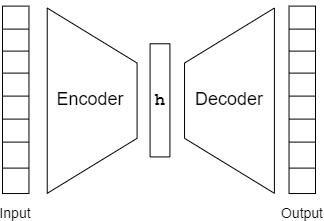
\includegraphics[width=0.6\textwidth]{AE.png}
    \caption{Minh họa ``Auto-Encoder''}
    \label{fig_AE}
\end{figure}

``Auto-Encoder'' được huấn luyện bằng cách cực tiểu hóa hàm lỗi là độ sai lệch giữa dữ liệu được tái tạo
với dữ liệu đầu vào. 
\begin{equation}
\label{AE_loss}
    L(x, g(f(x)))
\end{equation}
Các hàm để tính độ lỗi thường được dùng là ``Mean-square error'' hoặc ``Binary cross-entropy''.
Tương tự như các mạng nơ-ron khác, ``Auto-Encoder'' có thể được huấn luyện bằng phương pháp ``Gradient-descent''
với thuật toán lan truyền ngược (``back-propagation'').



Khi thiết kế mô hình, kiến trúc của encoder, decoder
và kích thước của véc-tơ \textbf{\textit{h}} được xem như những siêu tham số của mô hình.
Bằng các cách thiết lập khác nhau, mô hình sẽ có những tính chất khác nhau. 
``Auto-Encoder'' với encoder và decoder là những hàm phi tuyến (cụ thể là mạng nơ-ron với hàm kích hoạt phi tuyến)
với khả năng tính toán quá mạnh hay trường hợp kích thước của véc-tơ \textbf{\textit{h}}
lớn hơn hoặc bằng so với véc-tơ đầu vào sẽ dẫn đến mô hình chỉ học cách sao chép thay vì trích xuất các đặc trưng ẩn từ dữ liệu. 

Thông thường, một ``Auto-Encoder'' sao chép một cách ``hoàn hảo'' đầu vào thành đầu ra
sẽ không có nhiều ý nghĩa. Thay vào đó, ``Auto-Encoder'' được thiết kế với các ràng buộc để không thể
học cách sao chép ``hoàn hảo'' mà chỉ có thể sao chép gần đúng, từ đó ta hy vọng quá trình 
huấn luyện ``Auto-Encoder'' sẽ thu được véc-tơ biểu diễn ẩn có những thông tin hữu ích.

Từ véc-tơ biểu diễn ẩn thu được trong quá trình huấn luyện ``Auto-Encoder'', ta có thể áp dụng mô hình này
như một mô hình trích xuất đặc trưng ẩn từ dữ liệu, làm đầu vào cho các tác vụ khác. 
Hoặc véc-tơ biểu diễn ẩn này có thể áp dụng được trong các tác vụ giảm chiều dữ liệu hỗ trợ cho các tác vụ
lưu trữ, truy vấn, tìm kiếm.

    \subsection{``Undercomplete Auto-Encoder''}
    \label{chap2/subsec11}
    Như đã trình bày trước đó, việc sao chép đầu vào thành đầu ra của ``Auto-Encoder'' không mang nhiều ý nghĩa.
    Với mục đích thu được véc-tơ biểu diễn ẩn của dữ liệu thông qua quá trình huấn luyện, ta cần các ràng buộc để có được \textbf{\textit{h}}
    nhận các thuộc tính hữu ích khi thiết kế mô hình.
    
    Một cách ràng buộc để mô hình có thể học được các đặc trưng ẩn từ dữ liệu
    là giới hạn véc-tơ đặc trưng ẩn \textbf{\textit{h}} có kích thước nhỏ hơn đáng kể so với véc-tơ đầu vào;
    tính chất này được gọi là ``under-complete''.
    
    Mô hình ``Auto-Encoder'' với kích thước \textbf{\textit{h}} nhỏ hơn đáng kể so với kích thước của véc-tơ đầu vào
    được gọi là ``Undercomplete Auto-Encoder''. Việc giới hạn này sẽ buộc mô hình phải nắm bắt các đặc trưng
    nổi bật nhất. Đây cũng là kiến trúc đa số các mô hình ``Auto-Encoder'' thường hay được sử dụng.

    Quá trình huấn luyện ``Undercomplete Auto-Encoder'' cũng giống với mô hình ``Auto-Encoder'',
    ta cần cực tiểu hóa hàm lỗi (công~thức~\ref{AE_loss}) là độ sai lệch giữa dữ liệu được tái tạo
    với dữ liệu đầu vào.

    ``Undercomplete Auto-Encoder'' là mô hình tốt để sử dụng cho các tác vụ tiêu biểu của ``Auto-Encoder'' truyền thống
    như trích xuất đặc trưng, giảm chiều dữ liệu 
    bởi vì tính chất ``under-complete'' của mô hình giúp dễ dàng thu được véc-tơ biểu diễn ẩn mang những thông tin hữu ích.


    \subsection{Biến thể của Auto-Encoder: ``Denoising Auto-Encoder''}
    \label{chap2/subsec12}
    
    Hàm lỗi của một ``Auto-Encoder'' thông thường sẽ ``phạt'' một mức nhất định với các mẫu dữ liệu được tái tạo lại
    khác với dữ liệu đầu vào. Điều này vô hình chung khuyến khích việc 
    $ f \circ g $ là một hàm đồng nhất nếu khả năng tính toán của $f$ và $g$ cho phép. Nói đơn giản hơn, điều này là việc mô hình sao chép ``hoàn hảo'' đầu vào thành đầu ra của nó.
    Khi đó, véc-tơ biểu diễn ẩn sẽ không có các thông tin hữu ích. 

    Bằng cách thay đổi cách tính toán độ lỗi khi tái tạo lại, cụ thể là thêm nhiễu vào véc-tơ đầu vào, 
    sau đó tính toán độ lỗi là đầu ra được mô hình tái tạo lại so với đầu vào ban đầu như sau:
    \begin{equation}
        L(x, g(f(\tilde{x})))
    \end{equation}
    với 
    \begin{math} \tilde{x} \end{math}
    là véc-tơ đầu vào 
    \begin{math}
        x
    \end{math} 
    được thêm một độ nhiễu, ta có được mô hình ``Denoising Auto-Encoder'' (DAE) (hình~\ref{fig_DAE}). 
    \begin{figure}
        \centering
        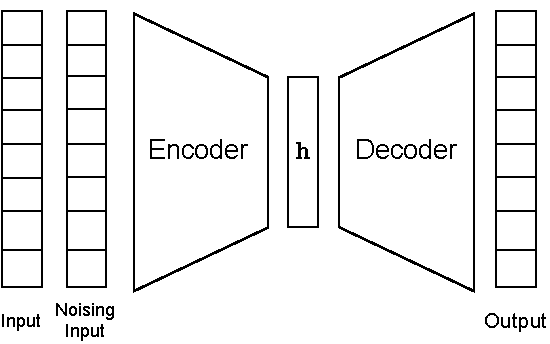
\includegraphics[width=0.6\textwidth]{DAE.pdf}
        \caption{Minh họa ``Denoising Auto-Encoder''}
        \label{fig_DAE}
    \end{figure}
    
    ``Denoising Auto-Encoder'' phải học cách khử độ nhiễu đã được thêm vào véc-tơ đầu vào, giảm khả năng sao chép của mô hình.

\section{Mô hình phát sinh dữ liệu ``Variational Auto-Encoder''} \label{chap2/sec2}
        \begin{figure}
            \centering
            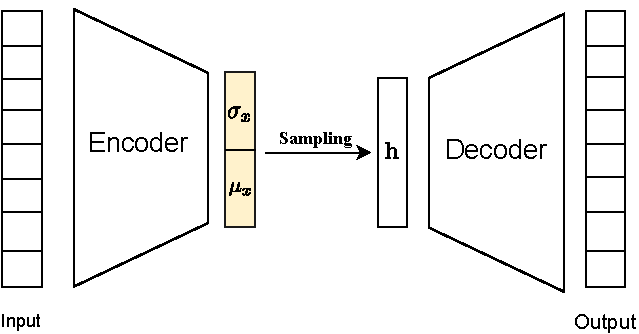
\includegraphics[width=0.6\textwidth]{VAE.pdf}
            \caption{Minh họa ``Variational Auto-Encoder''}
            \label{fig_VAE}
        \end{figure}
        ``Variational Auto-Encoder'' (VAE) là một biến thể đặc biệt của ``Auto-Encoder'' cơ bản (được minh họa trong hình~\ref{fig_VAE}). 
        VAE ngoài là một mô hình rút trích đặc trưng ẩn dựa trên phương pháp học không giám sát, còn là một mô hình phát sinh dữ liệu hiệu quả. 
        Phát sinh dữ liệu là việc mô hình có khả năng tạo ra những điểm dữ liệu `mới' dựa trên đặc trưng ẩn đã học được.
        Đây là một điểm khác biệt so với mô hình ``Auto-Encoder'' khi mà đặc trưng ẩn học từ ``Auto-Encoder'' cơ bản không thể được sử dụng để phát sinh. 
        Điều tạo nên sự khác biệt này là bởi đặc trưng ẩn có được từ VAE là một phân bố chứ không phải là một điểm dữ liệu cụ thể. 
        ``Auto-Encoder'' hay kể cả ``Denosing Auto-Encoder'', việc nhận dữ liệu đầu vào và trích xuất đặc trưng ẩn đều có thể được xem như là một phép chiếu dữ liệu ở chiều không gian cao lên một chiều không gian thấp hơn (thông thường thì kích thước của véc-tơ biểu diễn ẩn của một ``Auto-Encoder'' sẽ có tính chất ``under-complete'' như đã đề cập ở phần~\ref{chap2/subsec11}). 
        Do đó, ta có thể xem đặc trưng ẩn này như là một điểm dữ liệu ở một chiều không gian khác với số chiều thấp hơn thể hiện cho dữ liệu ban đầu. 
        Mặt khác, với VAE thì đặc trưng ẩn không còn là một điểm dữ liệu, thay vào đó sẽ là một ``phân phối xác suất''. 
        Phân phối xác suất thể hiện cho phân bố của một đại lượng, một biến ngẫu nhiên nào đó.
    
        Tuy nhiên, để làm rõ được sự hiệu quả của VAE trong việc phát sinh đặc trưng và phát sinh dữ liệu từ đặc trưng thì ta cần phải xét qua góc nhìn xác suất của mô hình này.
        Bản chất của một mô hình VAE là một mô hình đồ thị (graphical models) - là một mô hình dùng để giải thích các mối quan hệ giữa các biến ngẫu nhiên trong xác suất thống kê. Và nền tảng của mô hình là ``Variation Inference'' - là một phương pháp cũng thuộc lĩnh vực xác suất thống kê với mục đích có thể ``giải thích'' được dữ liệu mà ta không quan sát được từ những dữ liệu mà ta đã có. Tận dụng sức mạnh của mạng nơ-ron trong lĩnh vực học máy, các hàm số xác suất được thay thành các mạng nơ-ron. Và thông qua việc huấn luyện mô hình để tìm ra bộ trọng số tốt nhất để giải quyết bài toán được giả định mà mô hình cần giải quyết. 

        Do sự liên hệ chặt chẽ với lĩnh vực xác suất, ở mục này, chúng tôi sẽ trình bày về nền tảng xác suất liên quan với mô hình ``Variational Auto-Encoder'', bao gồm các khái niệm, định lý trong lĩnh vực xác suất thống kê để có thể dễ dàng trình bày nội dung của VAE ở mục tiếp theo, cũng như là cách huấn luyện cho mô hình VAE. 
        

    \subsection{Nền tảng xác suất của mô hình} \label{chap2/subsec21}
        
        Với sự tăng nhanh về số lượng dữ liệu có trên các nền tảng số thì nhu cầu cần một phương pháp có thể phân tích dữ liệu một cách tự động đang  càng ngày càng tăng theo.
        Mục tiêu của học máy đó là phát triển các phương pháp mà có thể tự động phát hiện các mẫu ``pattern'' trong dữ liệu.
        Các mô hình học máy tìm được những ``pattern'' này thông qua việc tìm các bộ tham số phù hợp với mô hình.
        Sau đó sử dụng những ``pattern'' vừa khám phá được để có thể dự đoán dữ liệu trong tương lai hoặc để thực hiện các mục đích khác như đưa ra các quyết định.
        Lý thuyết xác suất (``probability theory'') có thể được áp dụng cho bất kỳ vấn đề nào liên quan đến ``những điều chưa chắc chắn''. 
        Trong máy học, ``những điều chưa chắc chắn'' có thể là những sự thay đổi trong dữ liệu mà chúng ta chưa biết trước được, hay là những bộ tham số của mô hình.
        Gọi là chưa chắc chắn bởi vì ta không biết trước được và cũng không quan sát được về những điều này và ta không thể khẳng định hoàn toàn về những điều đó.
        Mô hình sẽ hoạt động như thế nào khi dữ liệu thay đổi? Liệu bộ tham số hiện tại của mô hình đã đủ tốt?
        Do đó học máy có liên quan khá là gần gũi với lĩnh vực xác suất thống kê và khai thác dữ liệu.

        
        Trên lý thuyết thì có ít nhất hai cách diễn giải của xác suất: ``diễn giải tần suất'' (frequentist interetation) và ``diễn giải bayesian''. Ở cách diễn giải thứ nhất thì xác suất được thể hiện thông qua việc thực hiện các thí nghiệm nhiều lần. Ví dụ như nếu ta thực hiện thí nghiệm tung đồng xu thì ta kì vọng rằng việc đồng xu xuất hiện mặt ngửa khoảng một nửa lần trong quá trình thực hiện. Còn ở cách diễn giải bayesian của xác suất thì thường được sử dụng để định lượng về ``những điều chưa chắc chắn''. Vậy nên ở góc nhìn này sẽ liên quan đến các thông tin hơn là việc lặp lại các thí nghiệm. Một trong những ưu điểm của cách diễn giải này đó là nó có thể được sử dụng để mô hình ``những điều chưa chắc chắn'' của sự việc/sự kiện mà ta đang quan tâm đến mà không có tần suất xuất dài hạn. Ví dụ liên hệ với các bài toán trong lĩnh vực học máy như chúng ta nhận một email và ta quan tâm đến việc tính phân phôi xác suất mà email vừa nhận là spam; hay trong bài toán chúng ta nhận thấy được một vật thể thông qua màn hình radar và ta muốn tính phân phối xác suất theo vật thể vừa được phát hiện chính xác là gì? một con chim, hay máy bay? Trong những trường hợp trên thì ý tưởng việc lặp lại các thí nghiệm sẽ không giúp ích cho chúng ta trong việc giải quyết các vấn đề nhưng với Bayesian thì điều này khá là tự nhiên và có thể được áp dụng để giải quyết bất kỳ vấn đề nào liên quan tới những ``điều không chắc chắn''.
        
        \subsubsection{Định lý Bayes và ứng dụng trong lĩnh vực học máy}
        Trong lĩnh vực ``máy học'' và ``thống kê Bayesian'', chúng ta thường quan tâm đến việc thực hiện các phép suy diễn dữ liệu ẩn ta không quan sát được khi cho trước các dữ liệu ta quan đã quan sát được.
        Ví dụ như ứng dụng một mô hình học máy trong việc phát hiện sản phẩm lỗi, khi ta đã có ghi nhận lại một số lượng dữ liệu mô tả của sản phẩm và đã biết được sản phẩm nào có lỗi hay không, đây chính là dữ liệu mà ta đã quan sát được. Điều mà ta quan tâm đến đó là mô hình có thể phát hiện được những ``pattern'' hay những đặc trưng quyết định đến việc xác định một sản phẩm có được xem là sản phẩm lỗi hay không, thì những ``pattern'' hoặc những đặc trưng này sẽ được xem là những dữ liệu ẩn.

        Giả sử rằng, ta có $a$ là biến ngẫu nhiên thể hiện cho dữ liệu ẩn mà ta không có dữ liệu về nó, và $b$ là biến ngẫu nhiên của dữ liệu mà ta có thể quan sát được.
        Theo đó, ta sẽ quan tâm đến việc tìm ra được giá trị $a$ cụ thể khi cho trước giá trị $b$. 
        Về xác suất, hay cụ thể ở đây, theo định lý Bayes, nếu ta có $p(a)$ là thông tin mà ta đã biết trước về biến ta không quan sát được $a$; và một số mẫu dữ liệu thể hiện mối quan hệ giữa $a$ và $b$ được thể hiện bởi $p(b|a)$, theo công thức Bayes, ta có:
        % $$p(a|b) = \frac{p(b|a)p(a)}{p(b)}$$\label{bayes}
        \begin{equation}
            \label{equal_bayes}
            p(a|b) = \frac{p(b|a)p(a)}{p(b)}
        \end{equation}

        Trong đó: 
        \begin{itemize}
            \item $p(a)$ được gọi là ``prior'', prior thể hiện cho ``kiến thức biết trước'' theo góc nhìn chủ quan ban đầu của chúng ta trước khi ta có bất kỳ về thông tin nào về liệu mà ta quan sát được.
            prior có thể được thể hiện thông qua một phân phối xác suất theo biến ẩn, nó có thể là phân phối xác suất bất kỳ sao cho phù hợp với chúng ta, nhưng một điều chúng ta cần phải đảm bảo đó là phân phối prior phải là có giá trị khác không trên tất cả các giá trị có thể xuất hiện của $a$, kể cả khi giá trị đó rất hiếm khi xảy ra.

            \item $p(b|a)$ là ``likelihood'', mô tả mối quan hệ giữa $a$ và $b$ liên quan với nhau như thế nào, và cụ thể thì nó là khả năng của việc xảy ra giá trị $b$ khi ta đã biết về dữ liệu ẩn $a$ cụ thể.
            
            \item Phân phối ``posterior'' $p(a|b)$ sẽ là giá trị mà ta quan tâm theo quan điểm của Bayes. Nó thể hiện rằng chúng ta có được thông tin gì về dữ liệu ẩn $a$ không quan sát được  khi ta có dữ liệu quan sát được là  $b$.
            
            \item $p(b)$ là ``evidence'' hay cũng còn được biết đến là ``marginal likelihood''. Phân phối thể hiện cho khả năng xảy ra của một giá trị B cụ thể. Ngoài ra evidence độc lập với $a$ nó còn có vai trò để chuẩn hoá cho posterior, có nghĩa là posterior sẽ có khoảng giá trị từ 0 đến 1.
        \end{itemize}
        Các đại lượng trong công thức~\ref{equal_bayes} được chú thích trong hình~\ref{fig_bayes}

        % Theo công thức trên thì
        %  $$p(y) = \int {p(y|x)p(x)\text{d}x = \mathrm{E}_X[p(y|x)]}$$ là ``marginal likelihood'' hay còn được gọi là ``evidence''. Trong công thức trên thì kí hiệu $\mathrm{E}$ thể hiện giá trị kỳ vọng của phân phối xác suất. Theo công thức của bayes thì, ``marginal likelihood'' độc lập với dữ liệu ẩn $x$, do đó ``marginal likelihood'' sẽ đóng vai trò đảm bảo giá trị của ``posterior'' sẽ được chuẩn hoá, có nghĩa là ``posterior'' sẽ có khoảng giá trị từ 0 đến 1. Tuy nhiên, với việc tính ``marginal likelihood'' là một giá trị tích phân, do đó thông thường việc tính toán giá trị chính xác cho ``marginal likelihood'' sẽ không dễ dàng. 

        \begin{figure}
            \centering
            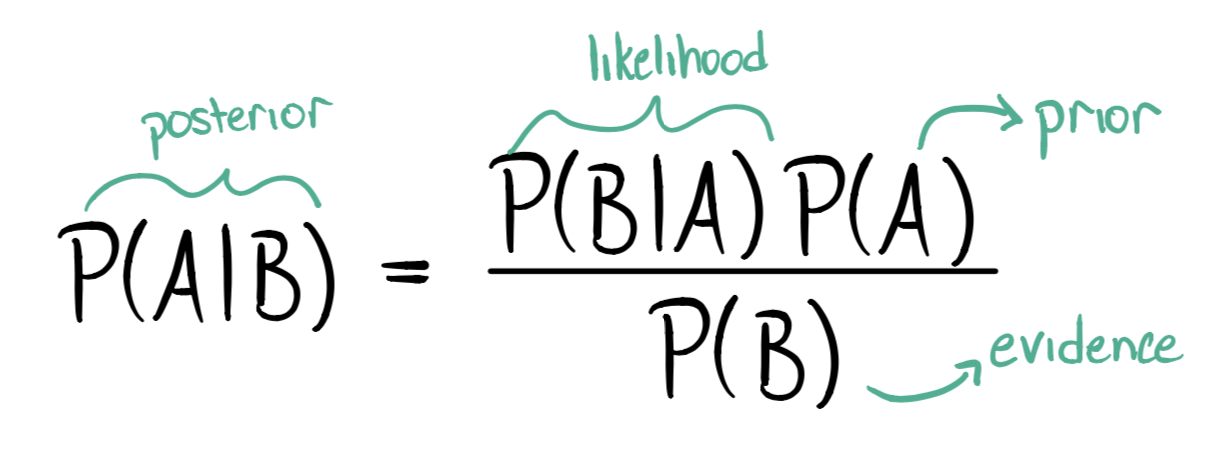
\includegraphics[scale=0.25]{bayes.png}
            \caption{Định lý ``Bayes''}
            \label{fig_bayes}
        \end{figure}
        
        \subsubsection{Khó khăn trong việc tính toán}
        Với góc nhìn này, ``posterior'' sẽ là giá trị mà chúng ta quan tâm đến, nó thể hiện mối quan hệ giữa ``prior'' của chúng ta và dữ liệu. 
        Việc tính toán ``posterior'' sẽ giúp chúng ta giải quyết các vấn đề trong thực tế.
        Theo công thức~\ref{equal_bayes}, để tính toán ``posterior'' ta cần phải có: ``prior'', ``likelihood'' và ``evidence''. Hai giá trị ở trên tử số (``prior'' và ``likelihood'') ta có thể dễ dàng xác định được trong hầu hết các trường hợp vì đó một phần là giả định của chúng ta về mô hình. Tuy nhiên, ở mẫu số ta cần tính:
        \begin{equation}
        \label{equal_evidence}
            p(b) = \int {p(b|a)p(a)\text{d}a = \mathbb{E}_a[p(b|a)]}    
        \end{equation}
        
        theo đó ta thấy được để tính được ``marginal likelihood'' thì ta cần tính biểu thức với dấu tích phân. Để tính giá trị này với dữ liệu ở chiều không gian thấp có thể không gặp nhiều khó khăn, nhưng khi tính toán ở những chiều không gian cao thì nó có thể trở thành một vấn đề nan giải. 
        Cụ thể ta thấy được rằng việc tính ``marginal likelihood'' sẽ thể hiện giá trị ``likelihood'' trung bình trên toàn bộ giá trị có thể xuất hiện của $a$, là những điều chưa chắc chắn trong mô hình, do đó $a$ ở chiều không gian càng cao thì việc tính toán càng trở nên phức tạp hơn. 

        Chúng ta cần chú ý thêm một vài khó khăn khác có thể phải đối mặt khi tính toán ``posterior'' đó là việc lấy ``tổ hợp'' khi dữ liệu là rời rạc thay vì giá trị liên tục. 
        Ở miền không gian liên tục thì ta có thể áp dụng hàm số trong lĩnh vực giải tích để tính toán, tuy nhiên trong những trường hợp mà chiều không gian của dữ liệu không liên lục, dữ liệu rời rạc thì việc tính toán sẽ còn phải xét thêm việc lấy tổ hợp dữ liệu. 

        Khi dữ liệu có số chiều lớn thì việc tính chính xác giá trị ``posterior'' trong thực tiễn thường sẽ là một việc cực kỳ khó khăn và bất khả thi và ta cần một vài kĩ thuật xấp xỉ thường được dùng để giải quyết việc tính ``posterior''. 

        \subsubsection{Bài toán Inference}
        Inference là một lớp bài toán để giải quyết vấn đề tìm hiểu về nhưng thứ mà ta biết được dựa trên những thứ mà ta đã biết. 
        Nói một cách khác thì bài toán này là tiến trình để có thể dưa ra kết luận giá trị ước lượng, hay khoảng tin cậy hoặc xấp xỉ một phân phối cho một ``biến ẩn'' (``latent variable'') thường được gọi là kết quả hay nhãn trong mẫu dữ liệu, dựa trên một vài các biến mà ta đã quan sát được thường được gọi là nguyên nhân hay dữ là dữ liệu đầu vào trong mẫu dữ liệu. 
        Ví dụ như ta có dữ liệu là hình ảnh của các đối tượng trong tự nhiên và có nhãn đi kèm mỗi ảnh, bài toán inference sẽ trả lời câu hỏi rằng nếu một tấm ảnh mới không có trước đó thì liệu ta có biết được nhãn của đối tượng trong ảnh hay không?. 

        ``Bayesian inferene'' là việc giải quyết bài toán inference dựa trên ``định lý Bayes''. Phương pháp Bayesian inference là một phương pháp trong lĩnh vực xác suất thống kê mà ở đó kiến thức biết được biết trước ``prior knowledge'' được mô hình hoá bởi một phân phối xác suất và được cập nhật mỗi khi có một quan sát mới và những thứ mà ta không chắc chắn hay không quan sát được sẽ được mô hình bởi một phân phôi xác suất khác. Một ví dụ kinh diển là về các tham số của ``Bayesian inference'', giả định rằng một mô hình mà dữ liệu $x$ được phát sinh từ một phân phối xác suất mà phân phối xác suất này được xác định bỏi các tham số $\theta$, tuy nhiên giá trị của $\theta$ thì ta chưa biết. Bên cạnh đó, ta giả định rằng, ta có một vài kiến thức được biết từ $\theta$ được gọi là ``prior knowledge'', nó có thể là phân phối xác suất $p(\theta)$. Sau đó, mỗi khi ta có một quan sát x mới, ta có thể cập nhật lại ``prior knowledge'' về tham số $\theta$ thông qua định lý Bayes theo công thức:

        trong đó 

        
        Bayesian Inference là một vấn đề thường được phải giải quyết trong các bài toán trong lĩnh vực xác suất thống kê tuy nhiên trong lĩnh vực học máy, nhiều phương pháp được xây dựng dựa trên việc giải quyết vấn đề Bayesian Inference. Ví dụ: ``Gaussian mixture models'' được dùng để giải quyêt bài toán phân lớp, hay ``Latent Dirichlet Allocation'' để giải quyết bài toán phân loại chủ đề văn vản. Và cả hai mô hình kể trên đều được xây dựng dựa trên việc giải quyết bài toán Bayes Inference.  

        % \subsubsection{Computational diffficulties}
        % Theo công thứ thì để tính toán ``posterior'' ta cần phải có: ``prior'', ``likelihood'' và ``evedience''. Hai giá trị ở trên tử số ta có thể dễ dàng ác định được trong hầu hết các trường hợp vì đó một phần là giả định của chúng ta về mô hình. Tuy nhiên, ở mẫu số ta cần tính:

        % để tính giá trị này với dữ liệu ở chiều không gian thấp có thể không gặp nhiều khó khăn, nhưng khi tính toán ở những chiều không gian cao thì nó có thể trở thành một vấn đề nan giải. Khi dữ liệu có số chiều lớn thì việc tính chính xác giá trị ``posterior'' trong thực tiễn thường sẽ là một việc cực kỳ khó khăn và bất khả thi và ta cần một vài kĩ thuật xấp xỉ thường được dùng để giải quyết việc tính ``posterior''. 

        % Chúng ta ca cần chú ý thêm một vài khó khăn khác có thể phải đối mặt khi giải quyết bài toán bayesian inference  như là việc lấy ``tổ hợp'' khi dữ liệu là rời rạc thay vì giá trị liên tục. 

        % % Bài toán bayesian inference thông thường sẽ xuất hiện trong các phương pháp học máy mà giả định rằng có một Graphical model và khi mà cho trước một vài dữ liệu mà ta có thể quan sát được và mục đích của chúng ta là muốn tái tạo lại dữ liệu ẩn của mô hình. Xét ví dụ trong phương pháp Latent Dircichlet Allocation, một phương pháp để xác định chủ đề của một đoạn văn bản. Ta được cho trước một tập ``từ điển'' với kích thước V từ và có T chủ đề có thể có, mô hình này giải định rằng
        % % \begin{itemize}
        % %     \item Với mỗi chủ đề, tồn tại một phân phối xác suất ``topic-word''  trên toàn bộ tập từ điển (giả định về prior)
        % %     \item Với mỗi đoạn văn bản, có tồn tại một phân phối xác suất ``document-topic'' trên toàn bộ tập các chủ đề (một giả định prior khác)
        % %     \item Với mỗi từ trong trong văn bản được lấy mẫu từ các phân phối giải định ở trên, cụ thể là đầu tiên chúng ta sẽ lấy mẫu một chủ đè từ phân phối xác suất ``document-topic'' của đoạn văn bản, tiếp theo, từ phân phối xác suất ``topic-word'' ta lấy mẫu một từ từ phân phối xác suất đi kèm với chủ đề được lấy mẫu ở bước trước. 
        % % \end{itemize}
        % % Tên của phương pháp này là xuất phát từ giả định Dirichlet pior của mô hình. Mục tiêu của mô hình là có thể suy diễn ``latent topic'' từ từ điển ta quan sát được cũng như là có thể phân rã chủ đề của từng đoạn văn bản. Kể cả khi nếu chúng ta không đi sâu vào chi tiết của mô hình LDA, chúng ta có thể nói một cách đại khái rằng với w là một véc-tơ các từ có trong từ điển và z là véc-tơ liên hệ với những từ đó, chúng ta muốn suy diễn được z dựa trên các quan sát từ w theo công thức bayes đó là:

        % %         $\text{có một công thức ở đây}$
 
        
        \subsubsection{Variational inference}
        Variational inference (VI) là một phương pháp thường hay được sử dụng để giải quyết bài toán ``Bayesian inference''.
        Phương pháp này sử dụng hướng tiếp cận là tìm ra xấp xỉ tốt nhất cho một phân phối xác suất bằng cách tìm ra giá trị của bộ tham số tốt nhất định nghĩa cho một phân phối khác, sao cho phân phối này sẽ ``gần'' với phân phối mà ta quan tâm. 
        
        Với phương pháp VI, đầu tiên ta sẽ tìm một phân phối xác suất có cùng ``họ'' (family) với phân phối xác suất mà ta quan tâm. 
        Một họ phân phối xác suất là tập các phân phối xác suất được định nghĩa bởi cùng một bộ tham số. 
        Ví như họ phân phối Gaussian sẽ được định nghĩa bởi $\mu$ là giá trị kỳ vọng (mean) và $\sigma$ là độ lệch chuẩn (standard deviation)
        Việc lựa chọn ``họ'' phân phối sẽ kiểm soát giữa độ phức tạp và độ chính xác của của phương pháp này. 
        Nếu ta giả định rằng dữ liệu tuân theo một phân phối đơn giản thì kết quả suy diễn được sẽ không quá chính xác nhưng có thể dễ dàng tìm được nghiệm tối ưu. Ngược lại nếu ta lựa chọn ``họ'' phân phối phức tạp thì sẽ khó tìm đươc nghiệm tối ưu nhưng kết quả suy diễn sẽ có kết quả tốt hơn. 

        Sau khi xác định được ``họ'' phân phối xác suất dùng để xấp xỉ phân phối xác suất mà chúng ta quan tâm thì việc tiếp theo là làm sao để tìm ra được xấp xỉ tốt nhất. 
        
        Giả sử rằng chúng ta cần sấp xỉ phân phối $p$ bởi một phân phối $q$ cùng thuộc họ phân phối $\mathcal{F}$.
        Chúng ta xét độ lỗi $\mathbb{E}(q,p)$ giữa hai phân phối xác suất $p$ và $q$, việc tìm ra bộ tham số tốt nhất được thể hiện bởi:
        \begin{equation}
        \label{equal_minErrorpq)}
            q^* = \text{arg}_{q\in\mathcal{F}} \text{min}\mathbb{E}(q,p)    
        \end{equation}
        

        Vậy trong bài toán variational inference thì làm sao để xác định hai phân phối xác suất có ``gần'' nhau hay không hay làm sao để xác định độ lỗi $\mathbb{E}(q,p)$. 
        Sự sai biệt Kullback-Leiber (KL) là một cách để tính mức độ lệch của một phân bố đối với một phân bố được chỉ định và thường được sử dụng để đo sự khác nhau giữa hai phân phối xác suất. 

        KL là môt thuật ngữ đến từ lĩnh lý thuyết thông tin, nó còn có tên gọi khác là entropy tương đối. Nói theo ngôn ngữ lý thuyết thông tin, nó đo lượng trung bình thông tin thêm vào nếu chúng ta mã hóa thông tin của phân bố $q$  thay cho mã hóa thông tin phân bố $p$.

        Nếu $p(x)$ và $q(x)$ là hai phân phối xác suất với $x$ là biến ngẫu nhiên bất kỳ, thì sự sai biệt KL sẽ được định nghĩa như sau:
        \begin{equation}
        \label{KLD}
            KL(q,p) = \mathbb{E}_q[\log q(x)] - \mathbb{E}_q[\log p(x)]    
        \end{equation}
        

        Sau khi xác định được một hàm lỗi để xấp xỉ phân phối xác suất mà chúng ta quan tâm $p$,  bởi phân phối $q$ thì bài toán sẽ trở thành việc tìm phân phối $q^*$ như sau:
        $$q^* = \text{arg}_{q\in\mathcal{F}} \text{min}\mathbb{E}_q[\log q(x)] - \mathbb{E}_q[\log p(x)] $$

        Việc tìm ra phân phối xác suất tốt nhất này trở thành một bài toán tìm nghiệm tối ưu do đó phương pháp này  có thể dễ dàng được áp dụng và mở rộng cho những trường hợp mà ta cần giải quyết một bài toán với quy mô dữ liệu lớn. 
        
        % \subsubsection{Kullback-Leiber Devergence}
        
            

        \subsubsection{ ``Maximum Likelihood Estimation''}
        \label{sec_mle}
        Trong lĩnh vực máy học, chúng ta sử dụng một mô hình để mô tả một tiến trình mà tổng hợp,
        phân tích tự động dữ liệu được thu thập để có thể giải quyết các vấn đề như tìm ra các đặc trưng,
        đưa ra các dự đoán dựa trên dữ liệu quan sát được.
        Xét ví dụ bài toán \textit{Hồi quy tuyến tính} (``Linear regression''),
        ta cần dự đoán giá trị $y$ dựa trên giá trị của véc-tơ $x$ theo công thức:
        \begin{equation}
        \label{equal_LR}
            y = wx + b
        \end{equation}
        Điều ta cần làm ở mô hình này là ``ước lượng'' giá trị tham số $w$ và $b$
        để mô hình có thể dự đoán giá trị $y$ một cách tốt nhất. 
        
        Với một mô hình máy học được mô tả bởi bộ tham số $\theta$, ta cần thực hiện ``ước lượng''
        bộ tham số $\theta$ sao cho mô hình có thể trả về kết quả tốt nhất. 
        Thay vì dự đoán một hàm số nào đó có khả năng ước lượng tham số tốt, ta cần một nguyên tắc để suy ra các hàm số cụ thể 
        cho các mô hình khác nhau.
        ``Maximum likelihood Estimation'' (MLE) là một công cụ phổ biến để thực hiện việc này.
        
        Xét tập dữ liệu gồm $m$ phần tử $\mathbb{X} = \{x_1,x_2,...,x_m\}$ là độc lập với nhau và được phát sinh từ một phân phối xác suất $p_{data}(x)$.
        Giả sử mô hình được mô tả bởi bộ tham số $\theta$. Khi đó, $p(x|\theta)$ là xác suất xảy ra sự kiện $x$ khi ta biết $\theta$.
        $p(x_1,x_2,...,x_m|\theta)$ chính là xác suất các sự kiện $x_1,x_2,...,x_m$ xảy ra đồng thời, xác suất đồng thời này được gọi là ``likelihood''.
        ``Likelihood'' của mô hình thể hiện khả năng mà bộ tham số của mô hình thể hiện mối quan hệ giữa dữ liệu mà ta có.
        Quá trình cực đại hóa ``likelihood'' là việc tối ưu khả năng mô hình thể hiện đúng nhất có thể mối quan hệ của dữ liệu.
        MLE là việc đi tìm bộ tham số $\theta$ sao cho likelihood là lớn nhất:
        \begin{equation}
        \label{equal_MLE}
                \theta = \max_{\theta} p(\mathbb{X};\theta)
        \end{equation} 
        
        Vì các phần tử trong $\mathbb{X}$ là độc lập và cố định, do đó công thức~\ref{equal_MLE} tương đương với:
        \begin{equation}
        \label{equal_MLE2}
            \theta = \max_{\theta} \prod_{i=1}^m p(x_i;\theta)
        \end{equation}        
        
        Bài toán MLE là quá trình tối ưu công thức~\ref{equal_MLE2}. Mà công thức này là một tích, thường thì việc tối ưu hóa một tích sẽ gặp rất nhiều khó khăn
        trong việc tính toán.
        Thay vào đó, ta tối ưu hàm logarit của ``likelihood'' bởi vì:
        \begin{itemize}
            \item logarit là một hàm đồng biến, ``likelihood'' sẽ lớn nhất khi logarit của `likelihood' là lớn nhất.
            \item logarit của một tích sẽ bằng tổng các logarit
        \end{itemize}
        Khi đó, bài toán MLE được đưa về bài toán ``Maximum log-likelihood Estimation''
        \begin{equation}
        \label{equal_loglikelihood}
            \theta = \max_{\theta} \sum_{i=1}^m \log(p(x_i;\theta))
        \end{equation}
        
        \textit{Gaussian likelihood} ám chỉ ``likelihood'' của mô hình với việc phân phối xác suất $p_{data}(x)$ thuộc ``họ'' Gaussian.
        Tương tự, các hàm likelihood khác cũng thường dùng trong các bài toán máy học là:
        \textit{Bernoulli likelihood, Multinomial likelihood}.
        
        

        
    


    \subsection{Mô hình ``Variational Auto-Encoder''} 
        \subsubsection{Mô hình xác suất}
        \textbf{\textit{Mô hình xác suất}} là một mô hình được dùng để mô tả một phân 
        phối xác suất hợp của dữ liệu bằng cách sử dụng một đồ thị để mô tả các biến 
        ngẫu nhiên tương tác với nhau trong phân phối xác suất. Ở đây 
        chúng tôi sử dụng từ ``đồ thị'' là một định nghĩa về cấu trúc 
        dữ liệu được mô tả trong lĩnh vực lý thuyết đồ thị. Đồ thị 
        bao gồm các đỉnh được kết nối trực tiếp với nhau thông qua 
        các cạnh. Vì cấu trúc của mô hình đươc mô tả bằng đồ thị cho 
        nên những mô hình này còn được gọi với một tên gọi khác là 
        ``Graphical model''. 
        Một graphical model sẽ thể hiện phân phối hợp như sau:
        $$p(x_1,x_2, .. ,x_N)$$
        trong đó $[x_1,x_2,..,x_N]$ là các đặc trưng dữ liệu, hoặc các tham số của mô hình,\dots Ví dụ như với bài toán phân loại thì một graphical model sẽ thể hiện cho phân phối $p(y,x, \theta)$ trong đó $x$ là đặc trưng đầu vào, $y$ là nhãn của dữ liệu và $\theta$ là trọng số của mô hình. 

        Graphical model cũng chính là một nhánh trong học máy, bằng cách thể hiện bài toán học máy dưới dạng một đồ thị. 
        Sự kết hợp giữa xác suất vào một mô hình học máy sẽ giúp mô hình ``giải thích'' vấn đề thực tế một cách tốt hơn. 
        Theo đó thì vấn đề cần quan tâm hoặc dữ liệu liên quan bởi các biến ngẫu nhiên. Và các biến ngẫu nhiên này chính là các đỉnh trong đồ thị và mối quan hệ giữa các đỉnh sẽ hình thành cạnh. Bằng cách thể hiện mối quan hệ giữa các biến dữ liệu bởi đồ thị ta dựa vào đó để có thể giải quyết các vấn đề mà chúng ta quan tâm. Ngoài ra bằng cách thể hiện bằng đồ thị, ta cũng thể hiện được tương quan giữa các biến dữ liệu, mà đa số các thuật toán máy học hiện nay thì tính tương quan giữa dữ liệu sẽ ảnh hưởng đến kết quả của mô hình. Dữ liệu có tính tương quan càng cao thì có thể sẽ ít đóng góp thêm ``thông tin'' cho mô hình thì có thể dẫn đến việc kết quả mô hình mang lại sẽ không cao. Do đó khi xây dựng thuật toán hay mô hình cho một vấn đề cụ thể, ta có thể áp dụng các kiến thức ta biết trước về lĩnh vực đó, về dữ liệu để có thể xác định các đặc trưng cho mô hình thông qua đồ thị. Ngoài ra việc sử dụng graphical cũng sẽ cung cấp một cái nhìn tổng quan về mô hình cũng như dữ liệu, từ đó việc phân tích, thiết kế và cài đặt cũng sẽ dễ dàng hơn.

        \subsubsection{Variational Auto-Encoder dưới góc nhìn xác suất}
        Với góc nhìn của một mô hình mạng nơ-ron thì ``Variational Auto-Encoder'' chỉ là một mạng nơ ron đơn giản với cấu trúc hai phần như mô hình ``Auto-Encoder'' tổng quát, gồm encoder và decoder. 
        Encoder được dùng để trích xuất đặc trưng ẩn từ dữ liệu, điểm khác biệt so với ``Auto-Encoder'' cơ bản là encoder của VAE sẽ là một phân phối xác suất.
        Và tương tự thì decoder sẽ là mạng nơ-ron cố gắng để tái tạo lại dữ liệu ban đầu từ đặc trưng ẩn.
        Hình \ref{fig_VAE} thể hiện kiến trúc cơ bản của mô hình variational Auto-Encoder.


        \begin{figure}
            \centering
            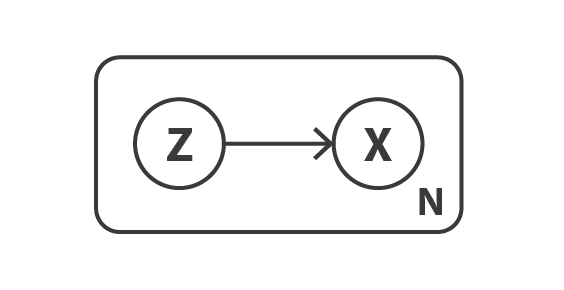
\includegraphics[scale=0.5]{dag_vae.png}
            \caption[Graphical model thể hiện cho mô hình ``Variational Auto-Encoder'']{Graphical model thể hiện cho mô hình ``Variational Auto-Encoder''. Dữ liệu quan sát được sẽ được giả định được phát sinh từ biến ẩn $z$} 
            \label{fig_dag_vae}
        \end{figure}

        Tuy nhiên để hiểu rõ hơn về nền tảng toán học cũng như xác suất trong mô hình chúng tôi sẽ trình bày mô hình VAE dưới góc độ là một mô hình xác suất.
        ``Variational Auto-enncoder'' là một mô hình đồ thị có hướng mô tả mối quan hệ giữa dữ liệu quan sát được và đặc trưng ẩn. Một đồ thị có hướng là một graphical model mà các đỉnh được kết nối với nhau có thứ tự. Có nghĩa là để có học được mẫu ở nút ``cha'' thì trước đó ta cần mô hình hoá đưọc dữ liệu ở nút con. Bên cạnh đó thì một graphical có hướng còn có tên gọi khác là ``Bayesian network''.
 
        
        Xét graphical model thể hiện cho mô hình VAE trong hình~\ref{fig_dag_vae}:
        ``Variational Auto-Encoder'' bao gồm một biến $x$ thể hiện cho dữ liệu, đây là biến dữ liệu quan sát được, và $z$ là biến ẩn thể hiện cho đặc trưng ẩn của dữ liệu. 
        Là một đồ thị có hướng do đó quá trình phát sinh dữ liệu của VAE được thực hiện qua các bước theo thứ tự như sau: 
        
        Với mỗi điểm dữ liệu: 
        \begin{itemize}
            \item Đặc trưng ẩn $z_i$ được lấy mẫu từ phân phối p(z)
            \item Điểm dữ liệu $x_i$ được lấy mẫu từ phân phối p(x|z)
        \end{itemize}

        Cụ thể, biến đặc trưng ẩn $z$ được chọn ra từ một phân phối ``prior'' $p(z)$ chính là những kiến thức ta biết trước ta biết trước hoặc là giả định của chúng ta về $z$. Điểm dữ liệu $x$ có một phân phối likelihood $p(x|z)$ thể hiện quan hệ giữa dữ liệu ta có với đặc trưng ẩn.
        Mô hình định nghĩa một phân phối hợp của dữ liệu và đặc trưng ẩn: $p(x,z)$. 
        Với quy tắc nhân trong xác suất, chúng ta có thể phân tách phân phối hợp trên thành ``prior'' và ``likelihood'' như sau: $p(x,z) = p(x|z)p(z)$. Đây chính là mục tiêu chính khi ta xét ``Variational Auto-Encoder'' dưới góc độ của xác suất.


        Mô hình này sử dụng phương pháp Variational inference được nhắc đến ở phần~\ref{chap2/subsec21} để tìm ra đặc trưng ẩn, đây cũng là lý do dẫn đến cái tên ``Variational Auto-Encoder''. Và VAE có thể được huấn luyện dựa trên các thuật toán  học dựa trên gradient truyền thống.
        
        
        Tiếp theo, ta xét đến việc suy diễn (inference) trong mô hình này. 
        Mục tiêu của việc suy diễn là tìm ra được một giá trị ``tốt'' thể hiện cho đặc trưng ẩn khi ta có các điểm dữ liệu, hay nói cách khác là ta tính ``posterior''.
        Theo công thức Bayes:
        \begin{equation}
        \label{equal_bayes1}
            p(a|b) = \frac{p(b|a)p(a)}{p(b)}
        \end{equation}
        theo như những gì đã trình bày ở những phần \ref{chap2/subsec21}, phần mẫu số 
        của công thức~\ref{equal_bayes1} được gọi là ``marginal likelihood''. 
        Và ``marginal likelihood'' sẽ không dễ dàng tính toán được một cách chính xác khi đặc trưng ẩn ở không gian có số chiều cao. 

        Do đó, phương pháp Vairational inference (VI) được áp dụng để xấp xỉ phân phối ``posterior'' $p(z|x)$ này.
        VI xấp xỉ posterior thông qua một phân phối xác suất có cùng họ phân phối $q_\lambda(z|x)$.
        Trong đó $\lambda$ thể hiện cho bộ tham số định nghĩa cho phân phối $q$, ví dụ nếu $q$ là  họ phân phối Gaussian thì $\lambda = (\mu;\sigma^2)$.
        
        Tiếp đến, ``Kullback-Leiber Devergence'' được sử dụng để xấp xỉ ``posterior'' 
        với:
        \begin{equation}
        \label{KLD1}
            \mathbb{KL}(q_\lambda(z|x) || p (z|x)) = \mathbb{E}_q[\log q_\lambda(z)] - \mathbb{E}_q[\log p(z|x)]
        \end{equation}
        trong đó các kỳ vọng đưọc lấy theo $q_\lambda(z)$.
        
        Biến đổi xác suất có điều kiện $p(z|x)$ ở công thức~\ref{KLD1}, ta có:
        \begin{equation}
        \label{KLD2}
            \mathbb{KL}(q_\lambda(z|x) || p (z|x)) =   \mathbb{E}_q[\log q_\lambda[(z|x)] - E_q[log p(x,z)] + \log p(x)
        \end{equation}
        Mục tiêu của chúng ta là tìm ra bộ tham số $\lambda$  sao cho tối thiểu được sự sai biệt trên. với $q^*$ là phân phối $q$ lý tưởng để xấp sỉ posterior thì ta có:
        \begin{equation}
        \label{equal_qlambda}
            q^*_\lambda(z|x) = \text{arg min}_\lambda KL(q_\lambda(z|x)|| p(x))
        \end{equation}        
        Tuy nhiên ta vẫn chưa có thể tính được trực tiếp bởi trong công thức thì vân còn xuất hiện $p(x)$, cho nên ``marginial likelihood'' vẫn không thể tính một cách trực tiếp.

        Vì không thể tính một cách trực tiếp ta xét một hàm số thay thế khác như sau:
        \begin{equation}
        \label{ELBO}
            ELBO(q_\lambda) = \mathbb{E}[\log p(z,x)] - \mathbb{E}[\log q_\lambda(z)]
        \end{equation}

        Biến đổi phân phối hợp $p(z,x)$ trong~\ref{ELBO}, ta lại có: 

        \begin{equation} \label{ELBO1}
            \begin{split}
                ELBO(q_\lambda) & = \mathbb{E}[\log p(z)]+ \mathbb{E}[\log p(x|z)] - \mathbb{E}[\log q_\lambda(z)]\\
                                & = \mathbb{E}[\log p(x|z)] - \mathbb{KL}( q_\lambda(z)|| p(z))
            \end{split}
        \end{equation}

        Công thức ~\ref{ELBO1} được gọi là ``evidence lower bound'' (ELBO).
        ELBO là trừ của sai biệt KL cộng với một lượng $\log p(x)$, bởi $\log p(x)$ là hằng số theo $q_\lambda(z)$.
        Bây giờ, việc cực đại ELBO sẽ tương đương với việc tối thiểu độ sai biệt KL.
        
        \label{trade_off}
        Bên cạnh đó, sau khi biến đổi mở rộng ELBO thì ta thấy rằng ELBO được tính từ 2 phần đó là kỳ vọng của likelihood và trừ KL giữa prior và phân phối sấp xỉ $q_\lambda(z)$.
        Với kỳ vọng của likelihood, nó thể hiện khả năng mô hình hoá dữ liệu còn sai biệt KL thì đảm bảo việc phân phối được xấp xỉ sẽ gần với prior của  dữ liệu.
        Đây chính là sự đánh đổi thường gặp trong những bài toán Bayesian inference, đánh đổi giữa khả năng mô hình hoá dữ liệu và việc đảm bảo phân phối được xấp sỉ hay cụ thể là đặc trưng ẩn sẽ gần với prior của chúng ta.

        % theo bất đẳng thức jensen thì Kullback-Leiber divergence luôn lớn hơn hoặc bằng không. 
        % Điều này có nghĩa rằng thay vì tối thiểu hoá KL thì ta sẽ thực hiện cực đại hoá ELBO.
        
        Sau khi nắm được lý thuyết nền tảng về xác suất của mô hình VAE, tiếp theo ta sẽ liên hệ với mạng nơ ron để thể hiện cho mô hình.
        Mục tiêu cuối cùng của chúng ta là tìm ra bộ tham số có thể xấp xỉ được posterior $ p(z|x,\lambda)$ bằng $q_\theta(z|x,\lambda) $ thông qua một mạng nơ ron thường được gọi là  ``inference network'' hay chính là encoder. Mạng này nhận đầu vào là dữ liệu $x$ và trả về kết quả là bộ tham số $\lambda$ thể hiện phân phối xác suất của đặc trưng ẩn. 
        Bên cạnh đó, sẽ có một mạng nơ ron được gọi là ``genetive network'' hay còn được biết đến là decoder thể hiện cho likelihood $p_{\phi}(x|z)$ của mô hình. 
        Tiếp theo đặc trưng ẩn sẽ được lấy mẫu từ phân phối xác suất trả ra từ encoder, đây chính là bước đầu tiên trong mô hình xác suất đã được nói ở  trên.
        Dữ liệu đầu vào của decoder là đặc trưng ẩn được lấy mẫu dựa trên phân phối của đặc trưng ẩn, và decoder sẽ cố gắng tái tạo lại dữ liệu ban đầu từ đặc trưng ẩn $z$, đây chính là bước thứ hai trong mô hình xác suất.
        
        Inference network và generative network sẽ có bộ tham số tương ứng là $\theta$ và $\phi$.
        Thông thường bộ tham số là các trọng số và bias trong một mạng nơ ron thông thường. 
        Mục tiêu của mô hình sẽ là cực đại hàm ELBO tương ứng như sau:
        \begin{equation}
        \label{ELBO2}
            ELBO(\theta,\phi) = \mathbb{E}_{q_\theta}(z|x)[\log p_\phi(x|z)] - \mathbb{KL}(q_\theta(z)||p(z))
        \end{equation}
        Để huấn luyện mô hình, ta có thể sử dụng những thuật toán học như ``gradient descent'' để có thể tìm ra bộ trọng số $\theta,\phi$.